\documentclass[tikz]{standalone}
\usetikzlibrary{positioning}
\usepackage{scalefnt}
\usepackage[ocr-a]{ocr}
\usepackage[T1]{fontenc}
\begin{document}
\normalfont\ocrfamily
\scalefont{2.62}
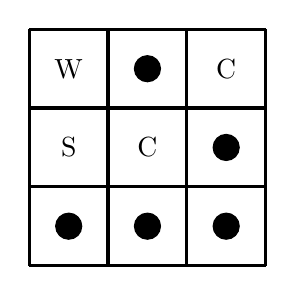
\begin{tikzpicture}[node distance=0.5, on grid, auto]
	\node (00) at (.5,-.5) {W}; \node[draw,circle,fill=black] (01) at (1.5,-.5) {}; \node (02) at (2.5,-.5) {C};
	\node (10) at (0.5,-1.5) {S}; \node (11) at (1.5,-1.5) {C}; \node[draw,circle,fill=black] (12) at (2.5,-1.5) {};
	\node[draw,circle,fill=black,radius=3] (20) at (.5,-2.5) {}; \node[draw,circle,fill=black] (21) at (1.5,-2.5) {}; \node[draw,circle,fill=black] (22) at (2.5,-2.5) {}; 
	
	\draw[step=1,very thick] (0,-3) grid (3,0);
\end{tikzpicture}
\end{document}